\documentclass[11pt]{beamer}  %% versione proiettore
%%\documentclass[11pt,handout]{beamer} %% versione stampa
\usepackage{lucidiJb-2ed}

\usepackage{relsize}

\mode<article>
{
  \usepackage{fullpage}
  \usepackage{hyperref}
}

\mode<presentation>
{
  \setbeamertemplate{background canvas}[vertical shading][bottom=red!10,top=blue!10]
  \usetheme{Ethereum}
  \usefonttheme[onlysmall]{structurebold}
}

\subtitle{Learning Ethereum}
\title{Wallets}
\institute{Universit\`a di Verona, Italy}
\date{January 2020}

\setbeamercovered{invisible}

\def\codesize{\smaller}
\def\<#1>{\codeid{#1}}
\newcommand{\codeid}[1]{\ifmmode{\mbox{\codesize\ttfamily{#1}}}\else{\codesize\ttfamily #1}\fi}

\begin{document}

\begin{frame}
  \titlepage
\end{frame}

\begin{frame}
  \frametitle{Wallets}

  \begin{greenbox}{}
    A wallet is a software application that keeps track of keys.
    It creates and broadcasts transactions signed with those keys.
  \end{greenbox}

  \bigskip

  \begin{greenbox}{Public key cryptography}
    Private and public keys come in pairs.
    Ethereum uses private keys to create
    digital signatures for transaction authentication.
    Hence EOAs are controlled by a private key.
  \end{greenbox}

  \bigskip

  \begin{redbox}{}
    Data are not natively encrypted in Ethereum!
  \end{redbox}

\end{frame}

\begin{frame}\frametitle{Private/public keys from random numbers}

  \begin{greenbox}{Private key}
    In principle, just a random sequence of $256$ bits.
  \end{greenbox}

  \bigskip

  \begin{redbox}{Cryptographically-secure random generators}
    Private keys should be generated by using a cryptographically-secure
    random generator, or otherwise keys might not really be randomly
    spread and might be more easily guessed.
  \end{redbox}

  \bigskip

  \begin{greenbox}{Public key}
    It is computed from the private key, through a one-way function
    called \emph{elliptic curve multiplication} (ECDSA).
  \end{greenbox}

  \begin{center}
    The generation of a private/public key pair does not require any
    centralized service. The probability of computing an already used key
    is negligeable.
  \end{center}

\end{frame}

\begin{frame}\frametitle{Ethereum representation of the keys}

  \begin{itemize}
    \item A private key are 256 random bits: 64 hexadecimal digits
    \item A public key is a couple of two 256 bit numbers: Ethereum
      uses \<0x04> followed by $64\times 2$ hexadecimal digits
  \end{itemize}

  \bigskip

  There are libraries for computing public keys from private keys:

  \begin{itemize}
  \item OpenSSL (\url{https://www.openssl.org})
  \item libsecp256k1 (\url{https://github.com/bitcoin-core/secp256k1})
  \end{itemize}

\end{frame}

\begin{frame}\frametitle{Cryptographic hash functions}

  \begin{greenbox}{Hash functions}
    Any function that can be used to map data of arbitrary size to data of
    fixed size.
  \end{greenbox}

  \bigskip

  \begin{greenbox}{Cryptographic hash function}
    A hash function with the following properties:
    \begin{enumerate}
    \item determinism
    \item verifiability (in linear time)
    \item noncorrelation (small change of input induces extensive change of hash)
    \item irreversibility (\emph{one-way})
    \item collision protection: difficult to compute two inputs that produce the same hash
    \end{enumerate}
  \end{greenbox}
  
\end{frame}

\begin{frame}\frametitle{Ethereum's cryptographic hash function}

  \begin{greenbox}{Keccak-256}
    Ethereum uses the Keccak-256 cryptographic hash function.
    It is the original algorithm that won the SHA-3 Cryptographic Hash
    Function Competition of 2007. NIST standardized it in a slightly
    modified way as SHA-3. However, the Ethereum team never trusted
    such modification and used the original agorithm.
  \end{greenbox}

  \bigskip

  \begin{redbox}{Keccak-256 or SHA-3?}
    You can still see blogs and even the source code of Ethereum refer
    to SHA-3. Despite of that, \underline{Etherem does not use SHA-3}, but the original
    Keccak-256 algorithm!
  \end{redbox}

\end{frame}

\begin{frame}\frametitle{Derivation of an Ethereum address from the private key}

  \begin{greenbox}{}
    Compute the public key (without leading \<0x04>),
    hash it with Keccak-256, keep only the last 20 bytes (160 bits).
  \end{greenbox}
  
  \begin{center}
    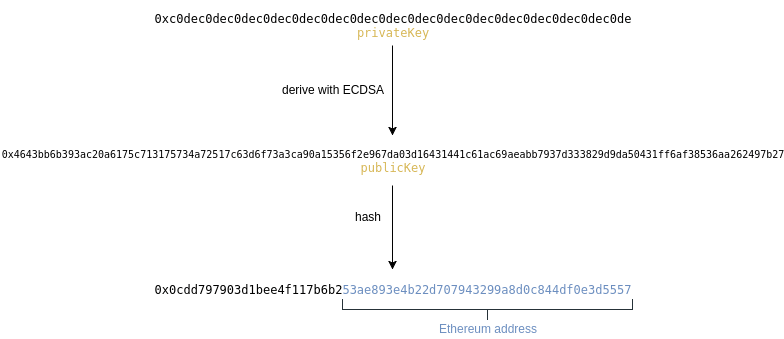
\includegraphics[width=\textwidth,clip=false]{pictures/ethereum-address-derivation.png}
  \end{center}

  \begin{center}
    No checksum!
  \end{center}

\end{frame}

\begin{frame}\frametitle{Checksummed address format: ICAP}

  \begin{greenbox}{}
    \<XE> + 2 characters of checksum + base-36 integer of up to 30 digits
  \end{greenbox}

  \bigskip

  \begin{greenbox}{}
    \begin{itemize}
    \item the base-36 integer can represent up to 155 bits, hence ICAP
      can only be used for addresses starting with a zero byte
    \item ICAP is compatible with IBAN
    \end{itemize}
  \end{greenbox}

  \bigskip

  \begin{greenbox}{Example}
    Ethereum address: \<0x001d3f1ef827552ae1114027bd3ecf1f086ba0f9>
    
    ICAP: \<XE60 HAMI CDXS V5QX VJA7 TJW4 7Q9C HWKJ D>
  \end{greenbox}

\end{frame}

\begin{frame}[fragile]\frametitle{Hex encoding with checksum in capitalization (EIP-55)}

  \begin{greenbox}{A backward compatible checksum injection}
    \begin{enumerate}
    \item use Keccak-256 to compute 64 hex digits from the uncapitalized Ethereum address
      (40 hex digits)
    \item capitalize each alphabetic address character if the corresponding hex digit
      of the hash is greater than or equal to \<0x8>
    \end{enumerate}
  \end{greenbox}

  \bigskip

  \begin{greenbox}{Example}
\begin{semiverbatim}
Address:   001d3f1ef827552ae1114027bd3ecf1f086ba0f9
Keccak256: 23a69c1653e4ebbb619b0b2cb8a9bad49892a8b9...
Result:    001d3{\color{red}F}1ef827552{\color{red}A}e111402{\color{red}B}7{\color{red}D}3{\color{red}ECF}1f086b{\color{red}A}0{\color{red}F}9
\end{semiverbatim}
  \end{greenbox}

  \bigskip

  \begin{greenbox}{Checking procedure of an EIP-55 encoded address}
    \begin{itemize}
    \item apply the above capitalization procedure to it
    \item the result must match the EIP-55 encoded address
    \end{itemize}
  \end{greenbox}

\end{frame}

\end{document}
